\documentclass[aspectratio=169, 10pt]{beamer}

% ==============================================================================
% PACKAGES & SYSTEM CONFIGURATION
% ==============================================================================
\usepackage[utf8]{inputenc}
\usepackage[T1]{fontenc}
\usepackage{lmodern}
\usepackage{amsmath, amssymb, amsfonts}
\usepackage{tikz}
\usetikzlibrary{shapes.geometric, arrows.meta, positioning, calc}
\usepackage{booktabs}
\usepackage{tabularx}
\usepackage{colortbl}
\usepackage{hyperref}

% ==============================================================================
% COLOR PALETTE (RFRecon AI Reference Theme)
% ==============================================================================
\definecolor{primaryblue}{RGB}{43, 57, 144}   % #2B3990 Royal / Deep Navy Blue
\definecolor{darknavy}{RGB}{20, 30, 70}       % #141E46 Deep Dark Navy (Footer Left)
\definecolor{midblue}{RGB}{43, 57, 144}       % #2B3990 Medium Royal Blue (Footer Center)
\definecolor{lightblue}{RGB}{70, 95, 175}     % #465FAF Slate Blue (Footer Right)
\definecolor{blockbg}{RGB}{240, 243, 250}     % #F0F3FA Light Tint (Diagrams)
\definecolor{textdark}{RGB}{25, 30, 45}       % #191E2D Deep Charcoal
\definecolor{accentteal}{RGB}{15, 118, 110}   % #0F766E Accent Teal
\definecolor{accentgreen}{RGB}{22, 163, 74}   % #16A34A Success Accent
\definecolor{accentred}{RGB}{220, 38, 38}     % #DC2626 Warning Accent

% ==============================================================================
% BEAMER TEMPLATES (Prevents Overleaf Scale, Overflow & White Gap Issues)
% ==============================================================================
\setbeamertemplate{navigation symbols}{}
\setbeamertemplate{headline}{} % Removes empty white space above frametitle

\setbeamercolor{normal text}{fg=textdark, bg=white}
\setbeamercolor{structure}{fg=primaryblue}
\setbeamersize{text margin left=0.6cm, text margin right=0.6cm}

% Edge-to-Edge Solid Top Banner
\setbeamertemplate{frametitle}{
  \nointerlineskip
  \begin{beamercolorbox}[wd=\paperwidth, ht=2.8ex, dp=1.2ex, leftskip=0.6cm, rightskip=0.6cm]{frametitle}
    \fontsize{13}{15}\selectfont\textbf{\insertframetitle}
  \end{beamercolorbox}
}
\setbeamercolor{frametitle}{bg=primaryblue, fg=white}

% 3-Part Footer with 3 Distinct Blue Shades & Centered Text (Visible on ALL slides)
\setbeamertemplate{footline}{
  \leavevmode%
  \hbox{%
    % Part 1: Project Name (Left)
    \begin{beamercolorbox}[wd=0.36\paperwidth, ht=2.5ex, dp=1.1ex]{footleft}%
      \centering\fontsize{7.5}{9}\selectfont\textbf{SDCS Digital Twin \& FDIA Defense}%
    \end{beamercolorbox}%
    % Part 2: Subject (Center)
    \begin{beamercolorbox}[wd=0.46\paperwidth, ht=2.5ex, dp=1.1ex]{footcenter}%
      \centering\fontsize{7.5}{9}\selectfont Software-Defined Communication Systems%
    \end{beamercolorbox}%
    % Part 3: Page Number (Right)
    \begin{beamercolorbox}[wd=0.18\paperwidth, ht=2.5ex, dp=1.1ex]{footright}%
      \centering\fontsize{7.5}{9}\selectfont\insertframenumber{} / \inserttotalframenumber%
    \end{beamercolorbox}%
  }%
  \vskip0pt%
}
\setbeamercolor{footleft}{bg=darknavy, fg=white}
\setbeamercolor{footcenter}{bg=midblue, fg=white}
\setbeamercolor{footright}{bg=lightblue, fg=white}

% Bullet & Numbering Badges (Matching RFRecon Reference Style)
\setbeamertemplate{itemize item}{\color{primaryblue}\scriptsize\raisebox{0.75pt}{$\blacktriangleright$}}
\setbeamertemplate{itemize subitem}{\color{primaryblue}\tiny\raisebox{0.75pt}{$\blacktriangleright$}}
\setbeamertemplate{enumerate item}{%
  \tikz[baseline=(char.base)]{%
    \node[shape=circle, fill=primaryblue, inner sep=1.1pt, text=white, font=\tiny\bfseries] (char) {\insertenumlabel};%
  }%
}

% TikZ Common Styles for Flowcharts Only
\tikzset{
  flowbox/.style={rectangle, rounded corners=2.5pt, draw=primaryblue, line width=0.8pt, fill=white, align=center, font=\fontsize{7}{8.5}\selectfont, inner sep=3.5pt},
  hwbox/.style={rectangle, rounded corners=2.5pt, draw=lightblue, line width=0.8pt, fill=blockbg, align=center, font=\fontsize{7}{8.5}\selectfont, inner sep=3.5pt},
  pipebox/.style={rectangle, rounded corners=2pt, draw=primaryblue, line width=0.7pt, fill=white, align=center, font=\fontsize{6.5}{7.5}\selectfont, inner sep=2.5pt},
  phasebox/.style={rectangle, rounded corners=3pt, draw=primaryblue, line width=0.9pt, fill=blockbg, align=center, font=\fontsize{7.5}{9}\selectfont, inner sep=4pt},
  arrow/.style={->, >=Stealth, line width=0.9pt, color=primaryblue}
}

% ==============================================================================
% DOCUMENT BEGIN
% ==============================================================================
\begin{document}

% ------------------------------------------------------------------------------
% SLIDE 1: TITLE SLIDE (Multi-Line Heading, Generous Margins, Tomorrow's Date)
% ------------------------------------------------------------------------------
\begin{frame}
  \begin{tikzpicture}[remember picture, overlay]
    \fill[primaryblue] (current page.north west) rectangle ([yshift=-2.85cm]current page.north east);
    \node[anchor=north, text=white, align=center, text width=0.85\paperwidth, yshift=-0.32cm] at (current page.north) {
      {\fontsize{15}{18}\selectfont\textbf{SDCS Digital Twin: Closed-Loop SDR}}\\[0.08cm]
      {\fontsize{14}{17}\selectfont\textbf{\& In-Band FDIA Threat Defense}}\\[0.12cm]
      {\fontsize{8.5}{11}\selectfont Real-Time Physical Telemetry, Adaptive Optimization \& Autonomous Mitigation}
    };
  \end{tikzpicture}
  
  \vspace{2.2cm}
  \begin{center}
    {\fontsize{11}{14}\selectfont\textbf{Team -- 13}}\\[0.20cm]
    {\fontsize{9}{11.5}\selectfont Mrityunjay.V -- CB.AI.U4CPS25029}\\[0.06cm]
    {\fontsize{9}{11.5}\selectfont Pavithiran.P -- CB.AI.U4CPS25035}\\[0.06cm]
    {\fontsize{9}{11.5}\selectfont Sanjit.K.R -- CB.AI.U4CPS25044}\\[0.06cm]
    {\fontsize{9}{11.5}\selectfont Vishal.B -- CB.AI.U4CPS25056}\\[0.22cm]
    {\fontsize{9}{11.5}\selectfont Software Defined Communication Systems}\\[0.05cm]
    {\fontsize{9}{11.5}\selectfont Amrita Vishwa Vidyapeetham}\\[0.18cm]
    {\fontsize{8.5}{10}\selectfont October 26, 2026}\\[0.22cm]
    {\fontsize{6.5}{8}\selectfont\texttt{\color{gray} GitHub: \href{https://github.com/floppa-png/SDCS-S3-Digital-Twin}{https://github.com/floppa-png/SDCS-S3-Digital-Twin}}}
  \end{center}
\end{frame}

% ------------------------------------------------------------------------------
% SLIDE 2: INTRODUCTION: WHY DIGITAL TWINS FOR SDR?
% ------------------------------------------------------------------------------
\begin{frame}{Introduction: Why Digital Twins for SDR?}
  \begin{itemize}\setlength{\itemsep}{12pt}\normalsize
    \item Real-world wireless channels change constantly due to thermal noise, multipath fading, and carrier drift.
    \item Traditional radios use a single fixed modulation: they waste data rate when the channel is good, and fail completely when the channel gets noisy.
    \item Manually reconfiguring radio settings during operation is too slow and impractical.
    \item A Digital Twin runs alongside the radio, continuously testing all candidate modulations in software to choose the best one.
    \item This creates an autonomous, self-healing communication link that adapts in real time.
  \end{itemize}
\end{frame}

% ------------------------------------------------------------------------------
% SLIDE 3: PROBLEM STATEMENT AND MOTIVATION
% ------------------------------------------------------------------------------
\begin{frame}{Project Problem Statement and Motivation}
  \textbf{\color{primaryblue}\large Problem Statement}\\[0.12cm]
  How can we design an SDR Digital Twin that monitors physical channel quality, predicts the optimal modulation in real time, auto-tunes transmission, explains its decisions, and defends against jamming attacks?
  
  \vspace{0.40cm}
  \textbf{\color{primaryblue}\large Why It Matters}\\[0.12cm]
  \begin{itemize}\setlength{\itemsep}{7pt}\small
    \item \textbf{Prevent Link Failure:} Automatically drops to more resilient modulations when channel quality degrades.
    \item \textbf{Maximize Throughput:} Automatically upgrades to higher-order modulations when conditions are clear.
    \item \textbf{Cyber-Physical Defense:} Detects malicious in-band jamming and diverts transmission to survive.
    \item \textbf{Hardware Validation:} Verifies closed-loop adaptation directly on ADALM-PLUTO SDR hardware.
  \end{itemize}
\end{frame}

% ------------------------------------------------------------------------------
% SLIDE 4: PROJECT OBJECTIVES (Enlarged, Rich Content, Well-Filled Slide)
% ------------------------------------------------------------------------------
\begin{frame}{Project Objectives}
  \begin{enumerate}\setlength{\itemsep}{9pt}\normalsize
    \item \textbf{Multi-Modulation Baseband Engine:} Generate and demodulate complex I/Q baseband signals for 7 core schemes (BPSK, QPSK, ASK, FSK, AM-DSBSC, AM-DSBTC, and FM).
    \item \textbf{Real-Time Digital Twin Optimization:} Continuously evaluate all 7 candidate modulations in parallel at 1~Hz using physical channel formulas to predict the winner.
    \item \textbf{Multi-Objective Scoring Function:} Formulate a composite score ($0-100$) balancing link reliability, data rate, bandwidth fit, and receiver power efficiency.
    \item \textbf{Over-the-Air SDR Hardware Link:} Transmit and receive live 2.4~GHz RF signals using the ADALM-PLUTO SDR interfaced with GNU Radio.
    \item \textbf{Explainable Web UI \& PDF Dossier:} Build an interactive web dashboard with live Physical Rationales and one-click printable PDF Link Dossier reports.
    \item \textbf{Cyber-Physical Jamming Defense:} Detect in-band swept jamming through multi-sensor trust scoring and automatically divert transmission to robust non-coherent FSK.
  \end{enumerate}
\end{frame}

% ------------------------------------------------------------------------------
% SLIDE 5: LITERATURE REVIEW (Centered, Balanced Line-Width)
% ------------------------------------------------------------------------------
\begin{frame}{Literature Review}
  \centering
  \scriptsize
  \begin{tabularx}{\linewidth}{p{2.5cm} p{1.6cm} p{2.1cm} X X}
    \toprule
    \textbf{Paper Title} & \textbf{Venue / Year} & \textbf{Technology} & \textbf{Key Contribution} & \textbf{Gap Addressed in Our Work} \\
    \midrule
    Digital Twin Enabled Cellular Management & IEEE Access, 2023 & SDR, Digital Twin & Predicts network KPIs and channel state in software. & Evaluated purely in simulation; lacks over-the-air SDR hardware-in-the-loop validation. \\
    \addlinespace
    Explainable Semantic Anomaly Characterization & IEEE JSAC, 2024 & Digital Twin, Explainable AI & Identifies channel anomalies and explains feature attribution. & Focuses on offline detection; lacks an automated real-time fallback mechanism during jamming. \\
    \addlinespace
    Modified Receiver in SDR for Modulation AMC & IEEE Trans. Comm., 2023 & ADALM-PLUTO, GNU Radio & Low-latency baseband receiver for modulation recognition. & Limited to digital schemes; does not support analog audio (AM/FM) or web-based live telemetry. \\
    \addlinespace
    Spectrum Sensing Using SDR for Cognitive Radio & IEEE Access, 2022 & SDR Testbed, Spectrum Sensing & Analyzes SDR hardware issues like DC offset and LO leakage. & Operates passively; does not score link quality or auto-tune transmitter settings in closed loop. \\
    \bottomrule
  \end{tabularx}
\end{frame}

% ------------------------------------------------------------------------------
% SLIDE 6: KEY DELIVERABLES AND SYSTEM WORKFLOW (Flowchart Boxes Around Workflow)
% ------------------------------------------------------------------------------
\begin{frame}{Key Deliverables and System Workflow}
  \begin{columns}[T]
    \begin{column}{0.48\linewidth}
      \textbf{\color{primaryblue}\normalsize Core SDR \& GNU Radio Pipeline}\\[0.15cm]
      \begin{itemize}\setlength{\itemsep}{7pt}\small
        \item Vectorized baseband engine generating 7 modulation schemes (digital and analog).
        \item GNU Radio flowgraph (\texttt{pluto\_hitl.grc}) streaming live over ADALM-PLUTO at 2.4~GHz.
        \item Barker-13 sync preamble and RRC pulse shaping for reliable packet detection.
        \item 150~kHz Digital IF offset to eliminate SDR hardware DC carrier leakage.
      \end{itemize}
    \end{column}
    
    \begin{column}{0.48\linewidth}
      \textbf{\color{primaryblue}\normalsize Twin Analytics, Explainability \& Security}\\[0.15cm]
      \begin{itemize}\setlength{\itemsep}{7pt}\small
        \item Digital Twin Engine evaluating all 7 candidate schemes in parallel at 1~Hz.
        \item 6-objective normalized fitness function producing a composite score ($0-100$).
        \item \textbf{Live Physical Rationale:} Explains why the winner was chosen in plain language.
        \item \textbf{Printable Link Dossier:} One-click export modal generating a PDF audit report.
        \item \textbf{In-Band FDIA Defense:} Automatic jamming detection with diversion to FSK.
      \end{itemize}
    \end{column}
  \end{columns}
  
  \vspace{0.40cm}
  \centering
  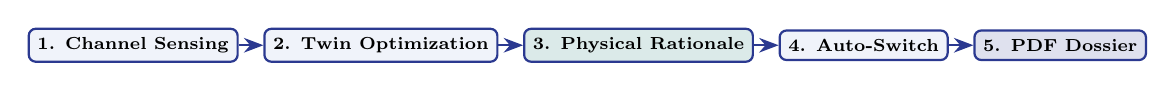
\begin{tikzpicture}[scale=0.90, every node/.style={transform shape}]
    \node[flowbox, fill=blockbg, font=\fontsize{7.5}{9}\selectfont] (b1) {\textbf{1. Channel Sensing}};
    \node[flowbox, fill=blockbg, font=\fontsize{7.5}{9}\selectfont, right=0.35cm of b1] (b2) {\textbf{2. Twin Optimization}};
    \node[flowbox, fill=accentteal!15, font=\fontsize{7.5}{9}\selectfont, right=0.35cm of b2] (b3) {\textbf{3. Physical Rationale}};
    \node[flowbox, fill=blockbg, font=\fontsize{7.5}{9}\selectfont, right=0.35cm of b3] (b4) {\textbf{4. Auto-Switch}};
    \node[flowbox, fill=primaryblue!15, font=\fontsize{7.5}{9}\selectfont, right=0.35cm of b4] (b5) {\textbf{5. PDF Dossier}};
    
    \draw[arrow] (b1) -- (b2);
    \draw[arrow] (b2) -- (b3);
    \draw[arrow] (b3) -- (b4);
    \draw[arrow] (b4) -- (b5);
  \end{tikzpicture}
\end{frame}

% ------------------------------------------------------------------------------
% SLIDE 7: SYSTEM ARCHITECTURE
% ------------------------------------------------------------------------------
\begin{frame}{System Architecture}
  \begin{columns}[T]
    \begin{column}{0.44\linewidth}
      \centering
      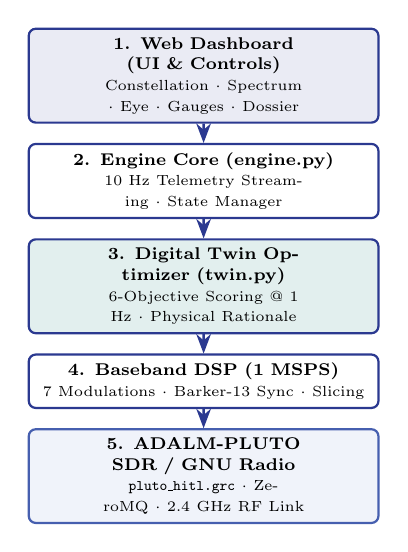
\begin{tikzpicture}[node distance=0.28cm, scale=0.88, every node/.style={transform shape}]
        \node[flowbox, fill=primaryblue!10, text width=4.8cm] (ui) {
          \textbf{1. Web Dashboard (UI \& Controls)}\\
          \fontsize{6.5}{7.5}\selectfont Constellation $\cdot$ Spectrum $\cdot$ Eye $\cdot$ Gauges $\cdot$ Dossier
        };
        \node[flowbox, below=of ui, text width=4.8cm] (eng) {
          \textbf{2. Engine Core (engine.py)}\\
          \fontsize{6.5}{7.5}\selectfont 10 Hz Telemetry Streaming $\cdot$ State Manager
        };
        \node[flowbox, fill=accentteal!12, below=of eng, text width=4.8cm] (twin) {
          \textbf{3. Digital Twin Optimizer (twin.py)}\\
          \fontsize{6.5}{7.5}\selectfont 6-Objective Scoring @ 1 Hz $\cdot$ Physical Rationale
        };
        \node[flowbox, below=of twin, text width=4.8cm] (dsp) {
          \textbf{4. Baseband DSP (1 MSPS)}\\
          \fontsize{6.5}{7.5}\selectfont 7 Modulations $\cdot$ Barker-13 Sync $\cdot$ Slicing
        };
        \node[hwbox, below=of dsp, text width=4.8cm] (hw) {
          \textbf{5. ADALM-PLUTO SDR / GNU Radio}\\
          \fontsize{6.5}{7.5}\selectfont \texttt{pluto\_hitl.grc} $\cdot$ ZeroMQ $\cdot$ 2.4 GHz RF Link
        };
        \draw[arrow] (ui) -- (eng);
        \draw[arrow] (eng) -- (twin);
        \draw[arrow] (twin) -- (dsp);
        \draw[arrow] (dsp) -- (hw);
      \end{tikzpicture}
    \end{column}
    
    \begin{column}{0.52\linewidth}
      \textbf{\color{primaryblue}\normalsize How the System Operates}\\[0.15cm]
      \begin{enumerate}\setlength{\itemsep}{6pt}\small
        \item \textbf{Web UI:} Displays live constellation, spectrum, and allows operator overrides.
        \item \textbf{Engine:} Coordinates background threads, logs events, and streams 10~FPS telemetry.
        \item \textbf{Twin Optimizer:} Uses physical formulas to predict the best modulation every second.
        \item \textbf{Baseband DSP:} Modulates and demodulates frames using NumPy at 1~MSPS.
        \item \textbf{Pluto SDR Link:} Transmits complex I/Q samples over the air at 2.4~GHz via GNU Radio.
      \end{enumerate}
    \end{column}
  \end{columns}
\end{frame}

% ------------------------------------------------------------------------------
% SLIDE 8: HARDWARE AND SOFTWARE SETUP
% ------------------------------------------------------------------------------
\begin{frame}{Hardware and Software Setup}
  \begin{columns}[T]
    \begin{column}{0.48\linewidth}
      \textbf{\color{primaryblue}\normalsize Hardware Setup}\\[0.15cm]
      \begin{itemize}\setlength{\itemsep}{8pt}\small
        \item \textbf{ADALM-PLUTO SDR:} Full-duplex software-defined radio operating from 70~MHz to 6~GHz.
        \item \textbf{2.4 GHz Whip Antennas:} Used for live over-the-air RF transmission and reception.
        \item \textbf{SMA Loopback Cable:} Used for calibrated hardware tests and baseline measurements.
        \item \textbf{Host Machine:} Laptop executing 1~MSPS baseband signal processing over USB 2.0.
      \end{itemize}
    \end{column}
    
    \begin{column}{0.48\linewidth}
      \textbf{\color{primaryblue}\normalsize Software Stack}\\[0.15cm]
      \begin{itemize}\setlength{\itemsep}{8pt}\small
        \item \textbf{GNU Radio 3.10:} Executes \texttt{pluto\_hitl.grc} flowgraph and XML-RPC control.
        \item \textbf{Python 3 \& NumPy:} Vectorized signal processing for baseband modulation and demodulation.
        \item \textbf{ZeroMQ:} Fast inter-process communication streaming samples between Python and GNU Radio.
        \item \textbf{Flask \& Socket.IO:} Real-time web server delivering 10~FPS telemetry to the dashboard.
      \end{itemize}
    \end{column}
  \end{columns}
\end{frame}

% ------------------------------------------------------------------------------
% SLIDE 9: METHODOLOGY: GNU RADIO SDR SIGNAL PROCESSING PATH
% ------------------------------------------------------------------------------
\begin{frame}{Methodology: GNU Radio SDR Signal Processing Path}
  \centering
  \textbf{\color{primaryblue}\small GNU RADIO HARDWARE-IN-THE-LOOP (HITL) BASEBAND PIPELINE}\\[0.15cm]
  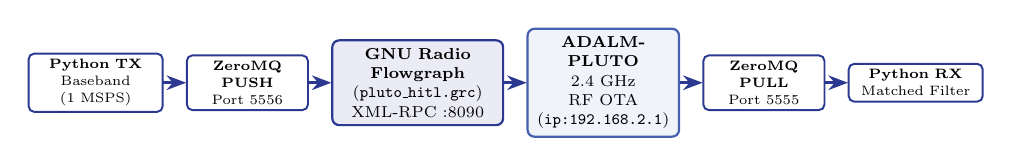
\begin{tikzpicture}[scale=0.82, every node/.style={transform shape}]
    \node[pipebox, text width=1.9cm] (pytx) {\textbf{Python TX}\\Baseband (1 MSPS)};
    \node[pipebox, right=0.35cm of pytx, text width=1.7cm] (zmq1) {\textbf{ZeroMQ PUSH}\\Port 5556};
    \node[flowbox, fill=primaryblue!10, right=0.35cm of zmq1, text width=2.4cm] (grc) {\textbf{GNU Radio Flowgraph}\\(\texttt{pluto\_hitl.grc})\\XML-RPC :8090};
    \node[hwbox, right=0.35cm of grc, text width=2.1cm] (pluto) {\textbf{ADALM-PLUTO}\\2.4 GHz RF OTA\\(\texttt{ip:192.168.2.1})};
    \node[pipebox, right=0.35cm of pluto, text width=1.7cm] (zmq2) {\textbf{ZeroMQ PULL}\\Port 5555};
    \node[pipebox, right=0.35cm of zmq2, text width=1.9cm] (pyrx) {\textbf{Python RX}\\Matched Filter};
    \draw[arrow] (pytx) -- (zmq1);
    \draw[arrow] (zmq1) -- (grc);
    \draw[arrow] (grc) -- (pluto);
    \draw[arrow] (pluto) -- (zmq2);
    \draw[arrow] (zmq2) -- (pyrx);
  \end{tikzpicture}
  
  \vspace{0.35cm}
  \begin{columns}[T]
    \begin{column}{0.48\linewidth}
      \textbf{\color{primaryblue}\normalsize GNU Radio Flowgraph Integration}\\[0.10cm]
      \begin{itemize}\setlength{\itemsep}{5pt}\small
        \item Receives transmit I/Q from Python over ZeroMQ port 5556.
        \item Sends received RF I/Q back to Python over ZeroMQ port 5555.
        \item Directly drives ADALM-PLUTO hardware buffers at 2.4~GHz.
        \item Exposes XML-RPC server (port 8090) for live gain and frequency tuning.
      \end{itemize}
    \end{column}
    
    \begin{column}{0.48\linewidth}
      \textbf{\color{primaryblue}\normalsize Hardware Engineering Fixes}\\[0.10cm]
      \begin{itemize}\setlength{\itemsep}{5pt}\small
        \item \textbf{150 kHz Digital IF Shift:} Bypasses Pluto's center LO DC leakage spike.
        \item \textbf{Reliable Streaming:} Sustains full-duplex 1~MSPS transfer without dropping samples.
        \item \textbf{Dual Execution:} Runs headless via native bridge or visually inside GNU Radio Companion.
      \end{itemize}
    \end{column}
  \end{columns}
\end{frame}

% ------------------------------------------------------------------------------
% SLIDE 10: METHODOLOGY: SUPPORTED MODULATION SCHEMES
% ------------------------------------------------------------------------------
\begin{frame}{Methodology: Supported Modulation Schemes}
  \centering
  \small
  \begin{tabularx}{\textwidth}{p{2.2cm} p{1.6cm} p{1.6cm} X}
    \toprule
    \textbf{Scheme} & \textbf{Category} & \textbf{Bits / Symbol} & \textbf{Key Characteristic \& When It Wins} \\
    \midrule
    \textbf{BPSK} & Digital & 1 bit/sym & Maximum noise margin ($\pm 90^\circ$); wins under extreme noise and low SNR. \\
    \addlinespace
    \textbf{QPSK} & Digital & 2 bits/sym & Doubles data rate within the same bandwidth; wins in cellular multipath channels. \\
    \addlinespace
    \textbf{ASK (OOK)} & Digital & 1 bit/sym & Simple diode envelope detection; wins when receiver power must be minimal. \\
    \addlinespace
    \textbf{FSK} & Digital & 1 bit/sym & Non-coherent dual-tone detection; wins under high Doppler drift and jamming. \\
    \addlinespace
    \textbf{AM-DSBSC} & Analog & --- & High power efficiency with suppressed carrier; wins for voice links. \\
    \addlinespace
    \textbf{AM-DSBTC} & Analog & --- & Transmitted carrier for simple diode detection; wins when frequency drifts. \\
    \addlinespace
    \textbf{FM} & Analog & --- & Constant envelope with noise suppression; wins for high-fidelity audio. \\
    \bottomrule
  \end{tabularx}
  
  \vspace{0.35cm}
  \centering\small
  \textit{Transmitter automatically scales symbol rate $R_s$ to fit the allocated channel bandwidth.}
\end{frame}

% ------------------------------------------------------------------------------
% SLIDE 11: DIGITAL TWIN SCORING AND AUTOPILOT
% ------------------------------------------------------------------------------
\begin{frame}{Digital Twin Scoring and Autopilot}
  \begin{columns}[T]
    \begin{column}{0.48\linewidth}
      \textbf{\color{primaryblue}\normalsize 6-Objective Composite Score ($0-100$)}\\[0.10cm]
      Combines 6 normalized sub-scores ($S_i \in [0, 1]$):
      \begin{itemize}\setlength{\itemsep}{4pt}\small
        \item \textbf{Reliability ($S_{\text{rel}}$):} Compares BER against target or output SNR.
        \item \textbf{Data Rate ($S_{\text{rate}}$):} Evaluates achieved throughput.
        \item \textbf{Bandwidth Fit ($S_{\text{bw}}$):} Penalizes signals that spill outside channel.
        \item \textbf{Power Margin ($S_{\text{pwr}}$):} Rewards operation safely above threshold.
        \item \textbf{Receiver Simplicity ($S_{\text{cplx}}$):} Rewards low-power diode detectors.
        \item \textbf{PAPR Efficiency ($S_{\text{papr}}$):} Rewards constant-envelope signals (FSK, FM).
      \end{itemize}
    \end{column}
    
    \begin{column}{0.48\linewidth}
      \textbf{\color{primaryblue}\normalsize Autopilot Closed-Loop Automation}\\[0.10cm]
      \begin{itemize}\setlength{\itemsep}{6pt}\small
        \item \textbf{1 Hz Twin Predictor:} Simulates all 7 candidates simultaneously in software to predict the winner.
        \item \textbf{Autonomous Switching:} Automatically commands the transmitter to switch to the highest-scoring scheme.
        \item \textbf{Anti-Ping-Pong Hysteresis:} Requires a 4.0~s dwell time and a 6-point hurdle to avoid rapid switching.
        \item \textbf{Safety Fallback:} If reliability drops sharply ($S_{\text{rel}} < 0.2$), total score is slashed by 50\% to force diversion.
      \end{itemize}
    \end{column}
  \end{columns}
\end{frame}

% ------------------------------------------------------------------------------
% SLIDE 12: WEB DASHBOARD, EXPLAINABILITY AND PRINTABLE DOSSIER
% ------------------------------------------------------------------------------
\begin{frame}{Web Dashboard, Explainability \& Printable Dossier}
  \begin{columns}[T]
    \begin{column}{0.48\linewidth}
      \textbf{\color{primaryblue}\normalsize Live Visual Telemetry (10 FPS)}\\[0.10cm]
      \begin{itemize}\setlength{\itemsep}{6pt}\small
        \item \textbf{Constellation Canvas:} Real-time I/Q display showing symbol scatter and noise in real time.
        \item \textbf{Welch PSD Spectrum:} 256-bin live FFT spectrum display with channel bandwidth mask.
        \item \textbf{Eye Diagram \& Oscilloscope:} Shows timing jitter and continuous baseband waveforms.
        \item \textbf{Radial Score Gauge:} Live 0--100 composite link score with letter grades (A+ to F).
      \end{itemize}
    \end{column}
    
    \begin{column}{0.48\linewidth}
      \textbf{\color{primaryblue}\normalsize Explainability \& Printable Dossier}\\[0.10cm]
      \begin{itemize}\setlength{\itemsep}{6pt}\small
        \item \textbf{Live Physical Rationale:} Real-time badge explaining the communication physics behind the twin's choice in plain words.
        \item \textbf{Printable Link Dossier (PDF):} One-click export modal generating a formal Link Dossier and Security Audit Report.
        \item \textbf{Scope Time-Window Filtering:} Operator can audit the Full Session (Boot) or recent windows (last 5m, 15m, 1h).
        \item \textbf{Complete Audit Records:} Exports uptime KPIs, hardware link state, attack mitigation stats, and event history.
      \end{itemize}
    \end{column}
  \end{columns}
\end{frame}

% ------------------------------------------------------------------------------
% SLIDE 13: CYBER-PHYSICAL SECURITY: IN-BAND FDIA DEFENSE (Three Trust Score Metrics)
% ------------------------------------------------------------------------------
\begin{frame}{Cyber-Physical Security: In-Band FDIA Defense}
  \centering
  \textbf{\color{primaryblue}\small IN-BAND FALSE DATA INJECTION ATTACK (FDIA) DEFENSE}\\[0.10cm]
  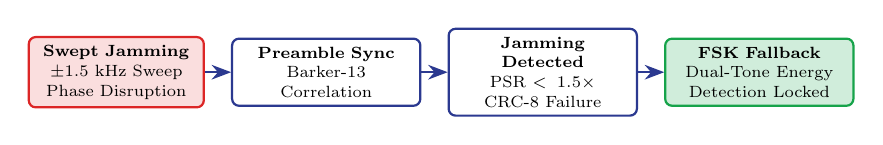
\begin{tikzpicture}[node distance=0.35cm, scale=0.84, every node/.style={transform shape}]
    \node[flowbox, draw=accentred, fill=accentred!15, text width=2.4cm] (jam) {\textbf{Swept Jamming}\\$\pm 1.5$ kHz Sweep\\Phase Disruption};
    \node[flowbox, right=0.4cm of jam, text width=2.6cm] (sync) {\textbf{Preamble Sync}\\Barker-13 Correlation};
    \node[flowbox, right=0.4cm of sync, text width=2.6cm] (det) {\textbf{Jamming Detected}\\PSR $< 1.5\times$\\CRC-8 Failure};
    \node[flowbox, fill=accentgreen!20, draw=accentgreen, right=0.4cm of det, text width=2.6cm] (fsk) {\textbf{FSK Fallback}\\Dual-Tone Energy\\Detection Locked};
    \draw[arrow] (jam) -- (sync);
    \draw[arrow] (sync) -- (det);
    \draw[arrow] (det) -- (fsk);
  \end{tikzpicture}
  
  \vspace{0.30cm}
  \begin{columns}[T]
    \begin{column}{0.48\linewidth}
      \textbf{\color{primaryblue}\normalsize 3 Sensors Evaluating Trust Score}\\[0.10cm]
      \begin{itemize}\setlength{\itemsep}{6pt}\small
        \item \textbf{1. Correlation Peak Ratio (PSR):} Measures Barker-13 correlation sharpness. Jamming pulls carrier phase and collapses PSR from $>3.5\times$ to $<1.5\times$.
        \item \textbf{2. CRC-8 Header Check:} Frame integrity validation. Phase interference causes bit flips and triggers immediate CRC failures.
        \item \textbf{3. Constellation Distortion (EVM):} Slicer error spikes as the swept jammer sweeps the band, crashing the Trust Score ($100\% \rightarrow <40\%$).
      \end{itemize}
    \end{column}
    
    \begin{column}{0.48\linewidth}
      \textbf{\color{primaryblue}\normalsize Autonomous Defense \& Recovery}\\[0.10cm]
      \begin{itemize}\setlength{\itemsep}{6pt}\small
        \item \textbf{Instant Fallback Trigger:} When Trust Score drops below threshold, the Digital Twin commands an automatic switch to FSK.
        \item \textbf{Immune to Phase Jamming:} Dual-tone FSK detects tone energy alone, completely ignoring carrier phase disruption caused by jamming.
        \item \textbf{100\% Link Recovery:} Restores clean, error-free communication while coherent schemes (BPSK, QPSK) remain blinded.
      \end{itemize}
    \end{column}
  \end{columns}
\end{frame}

% ------------------------------------------------------------------------------
% SLIDE 14: RESULTS: PRESETS AND WINNER REGIMES
% ------------------------------------------------------------------------------
\begin{frame}{Results: Presets and Winner Regimes}
  \centering
  \scriptsize
  \begin{tabularx}{\textwidth}{p{2.2cm} p{3.8cm} c c p{4.6cm}}
    \toprule
    \textbf{Preset} & \textbf{Channel Condition} & \textbf{Winner} & \textbf{Score} & \textbf{Physical Rationale} \\
    \midrule
    \texttt{deep\_space} & Low SNR ($-2$~dB), High Noise & \textbf{BPSK} & \textbf{97} & Maximum phase separation ($\pm 90^\circ$); survives deep thermal noise. \\
    \addlinespace
    \texttt{urban\_cellular} & Moderate SNR ($14$~dB), Limited BW & \textbf{QPSK} & \textbf{92} & Fits bandwidth limit while delivering double the data rate of BPSK. \\
    \addlinespace
    \texttt{leo\_doppler} & High Doppler ($600$~Hz) \& Frequency Drift & \textbf{FSK} & \textbf{95} & Non-coherent energy detection ignores carrier frequency drift. \\
    \addlinespace
    \texttt{iot\_tag} & Low Power Profile, Narrow Bandwidth & \textbf{ASK} & \textbf{95} & Simple diode envelope detection uses minimal power. \\
    \addlinespace
    \texttt{am\_broadcast} & Analog Audio, $11$~kHz Bandwidth & \textbf{AM-DSBTC} & \textbf{92} & Transmitted carrier allows simple envelope recovery despite drift. \\
    \addlinespace
    \texttt{coherent\_voice} & Analog Audio, Clean Channel & \textbf{AM-DSBSC} & \textbf{93} & Suppressed carrier maximizes transmission power efficiency. \\
    \addlinespace
    \texttt{fm\_broadcast} & Wide Bandwidth ($200$~kHz), High SNR & \textbf{FM} & \textbf{96} & Constant envelope suppresses background noise for clear audio. \\
    \addlinespace
    \texttt{fdia\_attack} & Swept Jamming \& Phase Spoofing & \textbf{FSK} & \textbf{94} & Energy detection ignores carrier phase corruption caused by jamming. \\
    \bottomrule
  \end{tabularx}
  
  \vspace{0.25cm}
  \centering\small
  \textbf{Key Finding:} Every modulation scheme wins legitimately in its natural operating regime.
\end{frame}

% ------------------------------------------------------------------------------
% SLIDE 15: KEY CHALLENGES AND PRACTICAL SOLUTIONS
% ------------------------------------------------------------------------------
\begin{frame}{Key Challenges and Practical Solutions}
  \begin{columns}[T]
    \begin{column}{0.48\linewidth}
      \textbf{\color{primaryblue}\normalsize Hardware Challenges}\\[0.10cm]
      \begin{itemize}\setlength{\itemsep}{8pt}\small
        \item \textbf{SDR Center DC Leakage Spike:} Direct conversion hardware creates a center carrier spike that distorts symbols.\\
        $\blacktriangleright$ \textit{Fix:} Applied a \textbf{150~kHz Digital IF shift}, moving the signal completely away from DC.
        \item \textbf{Carrier Frequency Drift:} Crystal frequency offsets between TX and RX cause constellation rotation.\\
        $\blacktriangleright$ \textit{Fix:} Implemented preamble-based frequency estimation to correct offset before demodulation.
      \end{itemize}
    \end{column}
    
    \begin{column}{0.48\linewidth}
      \textbf{\color{primaryblue}\normalsize Channel \& Streaming Challenges}\\[0.10cm]
      \begin{itemize}\setlength{\itemsep}{8pt}\small
        \item \textbf{Multipath Fading \& Doppler:} Rapid phase shifts cause deep nulls in coherent modulations.\\
        $\blacktriangleright$ \textit{Fix:} Twin evaluates channel degradation and falls back to robust non-coherent FSK.
        \item \textbf{Real-Time Streaming Stability:} USB streaming can drop samples if processing latency spikes.\\
        $\blacktriangleright$ \textit{Fix:} Vectorized DSP in NumPy at a fixed \textbf{1~MSPS} rate, ensuring zero buffer drops.
      \end{itemize}
    \end{column}
  \end{columns}
\end{frame}

% ------------------------------------------------------------------------------
% SLIDE 16: PROJECT TIMELINE AND EXECUTION ROADMAP
% ------------------------------------------------------------------------------
\begin{frame}{Project Timeline and Execution Roadmap}
  \centering
  \textbf{\color{primaryblue}\small 6-PHASE SYSTEM DEVELOPMENT ROADMAP}\\[0.20cm]
  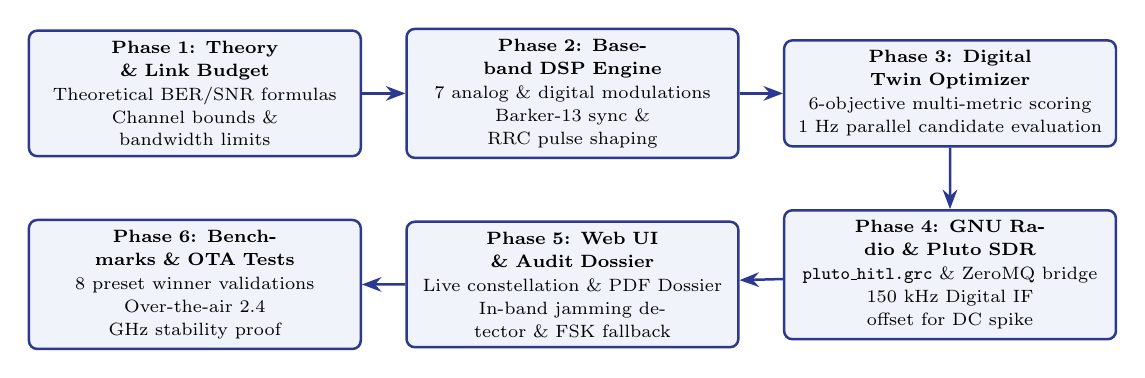
\begin{tikzpicture}[scale=0.92, every node/.style={transform shape}]
    % Row 1
    \node[phasebox, text width=4.3cm] (p1) {
      \textbf{Phase 1: Theory \& Link Budget}\\[0.05cm]
      \fontsize{7}{8}\selectfont Theoretical BER/SNR formulas\\
      Channel bounds \& bandwidth limits
    };
    \node[phasebox, right=0.6cm of p1, text width=4.3cm] (p2) {
      \textbf{Phase 2: Baseband DSP Engine}\\[0.05cm]
      \fontsize{7}{8}\selectfont 7 analog \& digital modulations\\
      Barker-13 sync \& RRC pulse shaping
    };
    \node[phasebox, right=0.6cm of p2, text width=4.3cm] (p3) {
      \textbf{Phase 3: Digital Twin Optimizer}\\[0.05cm]
      \fontsize{7}{8}\selectfont 6-objective multi-metric scoring\\
      1 Hz parallel candidate evaluation
    };
    % Row 2
    \node[phasebox, below=0.85cm of p1, text width=4.3cm] (p6) {
      \textbf{Phase 6: Benchmarks \& OTA Tests}\\[0.05cm]
      \fontsize{7}{8}\selectfont 8 preset winner validations\\
      Over-the-air 2.4 GHz stability proof
    };
    \node[phasebox, below=0.85cm of p2, text width=4.3cm] (p5) {
      \textbf{Phase 5: Web UI \& Audit Dossier}\\[0.05cm]
      \fontsize{7}{8}\selectfont Live constellation \& PDF Dossier\\
      In-band jamming detector \& FSK fallback
    };
    \node[phasebox, below=0.85cm of p3, text width=4.3cm] (p4) {
      \textbf{Phase 4: GNU Radio \& Pluto SDR}\\[0.05cm]
      \fontsize{7}{8}\selectfont \texttt{pluto\_hitl.grc} \& ZeroMQ bridge\\
      150 kHz Digital IF offset for DC spike
    };
    \draw[arrow] (p1) -- (p2);
    \draw[arrow] (p2) -- (p3);
    \draw[arrow] (p3) -- (p4);
    \draw[arrow] (p4) -- (p5);
    \draw[arrow] (p5) -- (p6);
  \end{tikzpicture}
  
  \vspace{0.35cm}
  \centering\small
  \textit{Multi-phase development ensured theoretical rigor before moving to live SDR hardware execution.}
\end{frame}

% ------------------------------------------------------------------------------
% SLIDE 17: REFERENCES (Standalone References Slide)
% ------------------------------------------------------------------------------
\begin{frame}{References}
  \footnotesize
  \begin{enumerate}\setlength{\itemsep}{7pt}
    \item X. Shen et al., ``Digital Twin Enabled Cellular Network Management and Prediction,'' \textit{IEEE Access}, vol. 11, pp. 24512--24528, 2023.
    \item Y. Lin et al., ``Explainable Semantic Wireless Anomaly Characterization for Digital Twins,'' \textit{IEEE JSAC}, vol. 42, no. 4, pp. 912--926, 2024.
    \item K. M. Addali et al., ``Modified Receiver Architecture in SDR for Real-Time Modulation Classification,'' \textit{IEEE Trans. Comm.}, 2023.
    \item J. Manco et al., ``Spectrum Sensing Using Software Defined Radio for Cognitive Radio Networks,'' \textit{IEEE Access}, 2022.
    \item J. G. Proakis and M. Salehi, \textit{Digital Communications}, 5th ed. McGraw-Hill, 2008.
    \item GNU Radio Project, \textit{GNU Radio: The Free \& Open-Source SDR Toolkit}, \url{https://www.gnuradio.org/}, 2024.
  \end{enumerate}
\end{frame}

% ------------------------------------------------------------------------------
% SLIDE 18: THANK YOU (Dedicated Standalone Slide)
% ------------------------------------------------------------------------------
\begin{frame}
  \vspace{1.0cm}
  \begin{center}
    {\fontsize{26}{32}\selectfont\textbf{\color{primaryblue} Thank You!}}\\[0.60cm]
    {\fontsize{14}{18}\selectfont Questions and Discussion}\\[0.80cm]
    {\fontsize{10}{13}\selectfont\textbf{Team -- 13}}\\[0.15cm]
    {\fontsize{9}{12}\selectfont Software Defined Communication Systems}\\[0.08cm]
    {\fontsize{9}{12}\selectfont Amrita Vishwa Vidyapeetham}\\[0.50cm]
    {\fontsize{8}{10}\selectfont\texttt{\color{gray} GitHub: \href{https://github.com/floppa-png/SDCS-S3-Digital-Twin}{https://github.com/floppa-png/SDCS-S3-Digital-Twin}}}
  \end{center}
\end{frame}

\end{document}
